\section{Equilibrium states}
%
\label{sec:equilibrium}

\subsection{The end state of tidal evolution}

Let us begin with a significantly simplified problem of tidal evolution. First,
consider a system consisting of just one planet and one star. Second, let us
assume that tides are allowed unlimited time to act. Third, let us ignore all
other processes that can change the system. Under these conditions, one of two
possible final states will eventually be reached. Either the two objects will
merge, or the system will end up in a state satisfying three simultaneous
properties: the orbit is circular, the planetary and stellar spin axes are
aligned with the orbital angular momentum, and the planet and star spin periods
are both equal to the orbital period.

Which of these two possibilities the system approaches depends on the initial
angular momentum available to the system. Since tides are purely internal
interactions within the system, they can only redistribute angular momentum, but
the total angular momentum vector must remain fixed. Let $M_\star$ and $M_p$ be
the masses of the star and planet, and $I_\star$ and $I_p$ their moments of
inertia.  If the two objects are to avoid merging, and reach a final
synchronized spin in a circular orbit with semimajor axis $a_f$, the final spin
angular velocities of both the star and the planet must be equal to the orbital
angular velocity, which by Kepler's third law is:

\begin{equation}
%
    \Omega_{orb} = \sqrt{\frac{G (M_\star + M_p)}{a_f^3}}
%
    \label{eq:orbital_angular_velocity}
%
\end{equation}

This gives the final angular momentum of the system as:

\begin{equation}
%
    L
%
    =
%
    \left(I_\star + I_p\right) \sqrt{\frac{G (M_\star + M_p)}{a_f^3}}
%
    +
%
    M_\star M_p \sqrt{\frac{G a_f}{M_\star + M_p}}
%
    \label{eq:equilibrium_angmom}
%
\end{equation}

The first term above is the sum of the spin angular momenta of the planet and
the star, and the second term is the orbital angular momentum.

\begin{figure}[t]
%
    \centering
%
    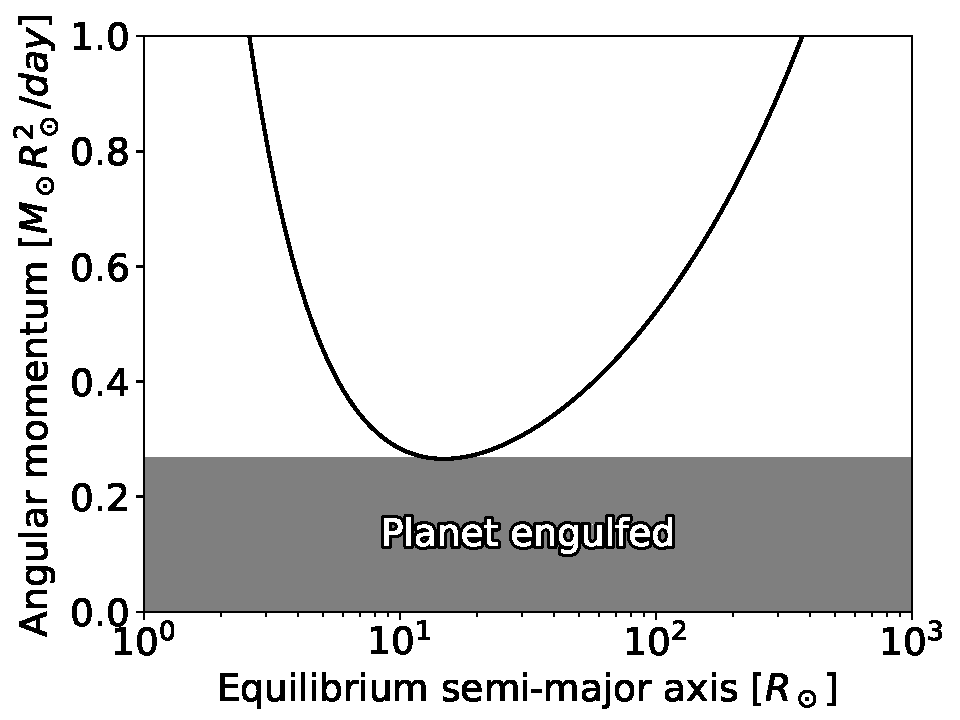
\includegraphics[width=0.5\textwidth]{equilibrium_angmom.pdf}
%
    \caption{
%
        The equilibrium angular momentum as a function of the equilibrium
        semimajor axis (Equation \eqref{eq:equilibrium_angmom}) for a
        star-planet system containing a star exactly like the present day Sun
        and a planet exactly like Jupiter.
%
    }
%
    \label{fig:equilibrium_angmom}
%
\end{figure}


From the above equation we see that $L \rightarrow \infty$ both as $a_f
\rightarrow 0$, and as $a_f \rightarrow \infty$, and that $L$ has a minimum
at a finite value of $a_f$. Figure \ref{fig:equilibrium_angmom} shows a graph of
equation \eqref{eq:equilibrium_angmom} for a Jupiter mass planet around a Solar
mass star. The minimum angular momentum for which equation
\eqref{eq:equilibrium_angmom} can be satisfied defines a critical value.  If the
initial angular momentum is smaller than this critical value, no equilibrium
state exists with the two objects surviving, hence the ultimate fate of a system
starting below this critical angular momentum is for the planet to be engulfed
by the star. If the initial angular momentum is larger than the minimum angular
momentum required by the final equilibrium state, then Eq.
\eqref{eq:equilibrium_angmom} allows us to calculate the final semimajor axis
and in turn the spin periods of the planet and the star.

Evidently, if the angular momentum exceeds the critical value, there are two
possible equilibrium states (there are two values of $a_f$ that satisfy Eq.
\eqref{eq:equilibrium_angmom}). From Equations
\eqref{eq:orbital_angular_velocity} and \eqref{eq:equilibrium_angmom} above one
can show that the solution with the smaller semimajor axis is an unstable
equilibrium, while the solution with the larger semimajor axis is in a stable
equilibrium. Physically, if an infinitesimal amount of angular momentum is
transferred from the orbit to the spin of the star (we can ignore the spin
angular momentum of the planet), both the spin and orbital angular velocities
will increase.  However, if a system starts with a semimajor axis equal to the
smaller of the two solutions, the orbital angular velocity will increase more
than the spin, which in turn will ensure tides will transfer even more angular
momentum from the orbit to the spin. If instead the system begins with the
larger semi-major axis solution, the orbital angular velocity will increase less
than the spin angular velocity and tides will work to undo the angular momentum
transfer.  Similar logic applies if one assumes an initial perturbation
transferring angular momentum from the spin to the orbit. In that case both the
orbital and spin angular velocities will decrease, but for the smaller semimajor
axis solution the orbital angular velocity will decrease faster, causing even
more angular momentum transfer from the spin to the orbit. As a result, if the
initial semi-major axis is larger than the smaller of the two solutions, tides
will drive the system toward the larger $a_f$, slower spinning, solution. If the
systems starts interior to the smaller of the two solutions, tides will cause
orbital decay until the planet is destroyed.

In practice, the simplifying assumptions we made above are often violated. Many
exoplanet systems have multiple planets, or even multiple stars. These extra
objects can perturb the orbit, maintaining non-zero eccentricity in spite of
tides. A particularly common situation that arises involves a pair or more
planets in what are called low order mean motion resonances. This mouthful of a
term refers to the situation where a small integer times the orbital period of
one planet is very close to another small integer times the orbital period of
another planet. An example of such mean motion resonance in our own solar system
are three of the four major satellites of Jupiter, where the orbital periods of
Io, Europa, and Ganymede are in a 1:2:4 ratio. Because planets in such
configurations repeatedly get closest to each other in the same place in their
orbit, the gravitational interactions between such planets are particularly
effective in exciting their orbital eccentricities. This excitation can compete
with tidal circularization, maintaining non-zero eccentricity. This prevents
tides from achieving the above equilibrium state. Instead, it can be shown
mathematically that in many situations, as tidal dissipation removes energy from
the systems, the resonant chain of planets will be maintained, causing all
planets to migrate inward together. This could cause the eventual engulfment of
some of the planets by the star even if the initial angular momentum is
sufficient according to the above criterion. In our own solar system, this
common migration seems to occur for Io, Europa, and Ganymede. Except in this
case the system of satellites moves outward rather than inward, because
Jupiter's spin period is shorter than even the shortest period orbit (that of
Io).

Even for a system of just a single planet and a single star, the assumption that
angular momentum is conserved may not hold. In particular, Sun-like stars
continuously lose angular momentum throughout their lifetime. This loss of
angular momentum gets larger the faster the star spins. Tides are generally only
important for orbital periods of order few days or less. In that case, the
equilibrium state described above will correspond to very fast stellar spin, ten
or more times faster than the present day spin of the Sun. At these spin rates,
the loss of angular momentum is significant enough to keep the orbit shrinking,
even if tides keep the system in a circular orbit and the stellar spin
synchronized with the orbit. This should not occur for higher mass stars, since
they appear to not experience appreciable angular momentum loss.

Finally, tides do not have unlimited time to act. Stars have finite lifetimes,
so even for an isolated system with just two objects, the equilibrium state may
not be reached before the star runs out of nuclear fuel and stars expanding.
This may result in the demise of the planet much sooner than due to tides alone.

\subsection{Spin-orbit locking in eccentric systems}

On their way to the synchronized and circularized state described above, planets
may find themselves crossing orbital configurations where the rate of tidal
evolution slows down dramatically. These quasi-equilibrium states require a
significantly eccentric orbit. For circular orbits, the time dependence of the
tidal forces experienced by any point within the planet or the star are simple
sine waves with a fixed frequency equal to twice the difference between the spin
and orbital angular velocity of the corresponding object. As already discussed
above, the direction of tidal evolution switches as this frequency crosses zero.

For eccentric orbits, the time dependence of the tidal forcing is more
complicated. Let us break up the problem into two parts. First, consider a
non-rotating object in an eccentric orbit. As already discussed above, we can
calculate the average effect of tides over a single orbit, ignoring the changes
in the orbit or the spin of the objects. Under this approximation, the tidal
forcing experienced by any part of a non-spinning object will be periodic with
the orbital period. As a result, we can think of the tidal forcing as a discrete
Fourier series of multiple tidal waves, with frequencies $m' \Omega_{orb}$,
where $\Omega_{orb}$ is the orbital frequency and $m'$ is an integer. If we now
include the rotation of the object with angular velocity $\Omega_{spin}$ and
assume its axis of rotation is aligned with the orbital angular momentum, each
of these waves will have its frequency shifted by $2\Omega_{spin}$, giving us a
series of tidal waves with frequencies $\Omega_{tide} = m' \Omega_{orb} - 2
\Omega_{spin}$. The factor of two comes from the fact that there are two tidal
bulges, one on the side facing the companion object and one on the opposite
side. In principle, for non-circular orbits, tidal waves exist for arbitrarily
large $m'$, though their amplitude becomes negligible as $m'\rightarrow\infty$.
Even more generally, if we now allow the axis of rotation to have any
orientation relative to the orbit, we end up with an even more general series of
tidal waves with frequencies:

\begin{equation}
%
    \Omega_{tide} = m' \Omega_{orb} - m \Omega_{spin},
%
    \quad m' \in \mathbb{Z},\quad m \in \left\{0, 1, 2\right\}
%
\end{equation}

At this point we need to introduce another simplifying assumption. Namely, we
will assume that the tidal perturbations are weak enough so we do not need to
worry about interactions between the separate tidal waves and instead we can
calculate the tidal torque and power each wave applies to the orbit separately
and calculate the evolution by simply adding these up.

Just like for the single tidal term of aligned circular orbits, the tidal torque
from each of these tidal terms changes its sign as the frequency of that term
crosses zero. If the amplitude of the tidal term for a given $m,m'$ is large
enough and the increase in dissipation as the frequency moves away from zero is
sufficiently steep, this change in the sign of the tidal torque introduces the
possibility that the spin of the object can be locked in a frequency close to
$\Omega_{spin}=\frac{m'}{m} \Omega_{orb}$. This can happen if the tidal torque
of that particular tidal term is large enough to cancel the combined torques of
all other terms. As the relative amplitudes of the different tidal terms depend
on the eccentricity, the set of frequencies at which the spin of the object can
be locked depends on the eccentricity of the orbit. The closer the orbit is to
circular the smaller the amplitude of the tidal terms with large $m'$, and hence
fewer terms will have sufficient amplitudes to hold the spin in a locked state.

In principle, both the planet and the star spin for eccentric systems can be
locked in one of these states. In our own Solar system, Mercury is in such a
spin-orbit locked state, with $m'=3$ and $m=2$, i.e. executing three revolutions
for every two orbital periods. It is likely that at least some exoplanets in
short orbital periods are also locked in similar states, as long as their orbits
have sufficient eccentricity to support the lock. Unfortunately, so far we have
not found a way to measure the spin of exoplanets, so we do not have a way of
observing this effect directly.

It is important to note that, even though the overall tidal torque is close to
zero if an object is in one of these pseudo-equilibrium states, tides in that
object can still contribute to the evolution of the orbit, since energy will
still be dissipated. The only truly stable tidal configuration is a circular
orbit with the spins of both objects synchronized with the orbit and their
equatorial planes coinciding with the orbital plane. And as pointed out above,
in the presence of non-tidal processes, even that may not be a configuration
which can last indefinitely.
